% Created by tikzDevice version 0.12.3.1 on 2022-04-28 14:33:47
% !TEX encoding = UTF-8 Unicode
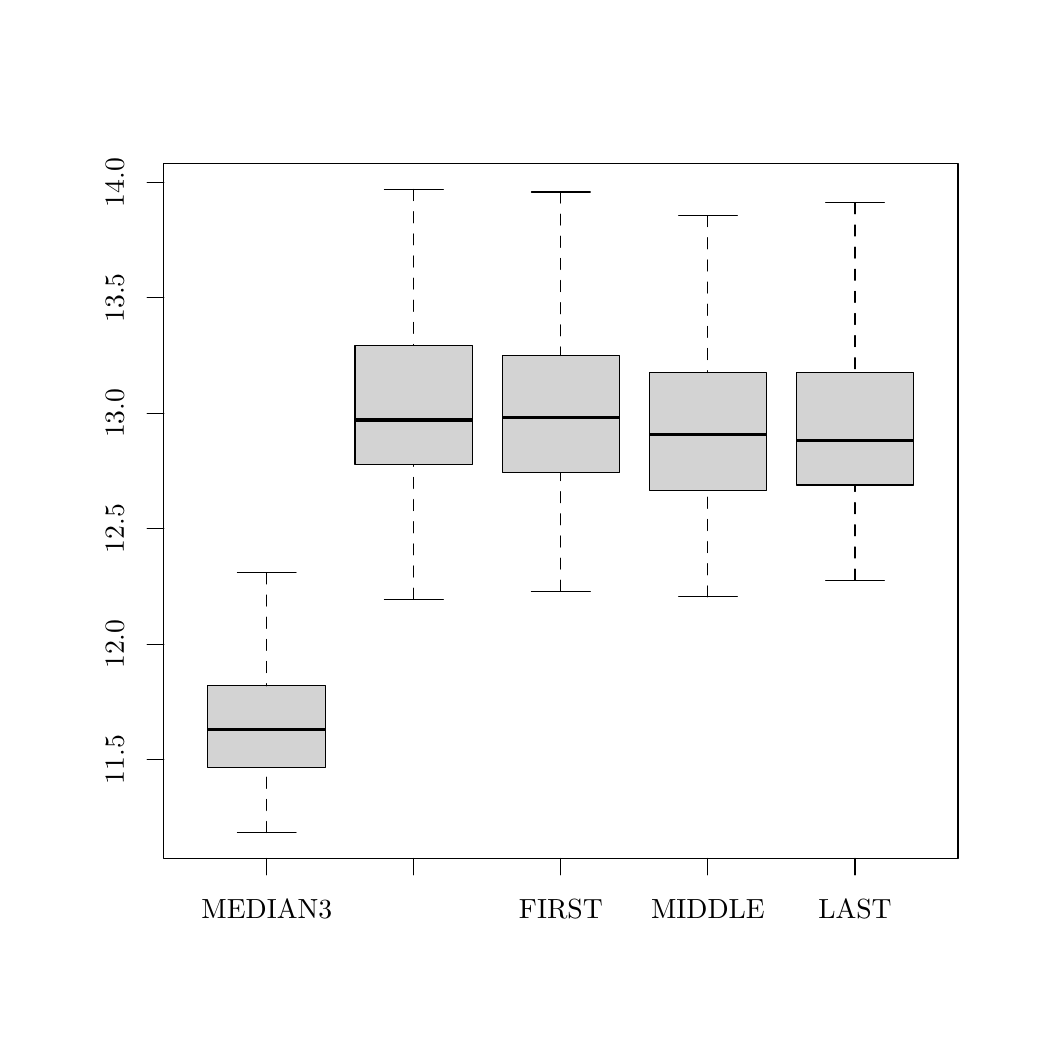
\begin{tikzpicture}[x=1pt,y=1pt]
\definecolor{fillColor}{RGB}{255,255,255}
\path[use as bounding box,fill=fillColor,fill opacity=0.00] (0,0) rectangle (361.35,361.35);
\begin{scope}
\path[clip] ( 49.20, 61.20) rectangle (336.15,312.15);
\definecolor{fillColor}{RGB}{211,211,211}

\path[fill=fillColor] ( 65.14, 94.04) --
	(107.65, 94.04) --
	(107.65,123.51) --
	( 65.14,123.51) --
	cycle;
\definecolor{drawColor}{RGB}{0,0,0}

\path[draw=drawColor,line width= 1.2pt,line join=round] ( 65.14,107.70) -- (107.65,107.70);

\path[draw=drawColor,line width= 0.4pt,dash pattern=on 4pt off 4pt ,line join=round,line cap=round] ( 86.40, 70.49) -- ( 86.40, 94.04);

\path[draw=drawColor,line width= 0.4pt,dash pattern=on 4pt off 4pt ,line join=round,line cap=round] ( 86.40,164.33) -- ( 86.40,123.51);

\path[draw=drawColor,line width= 0.4pt,line join=round,line cap=round] ( 75.77, 70.49) -- ( 97.02, 70.49);

\path[draw=drawColor,line width= 0.4pt,line join=round,line cap=round] ( 75.77,164.33) -- ( 97.02,164.33);

\path[draw=drawColor,line width= 0.4pt,line join=round,line cap=round] ( 65.14, 94.04) --
	(107.65, 94.04) --
	(107.65,123.51) --
	( 65.14,123.51) --
	cycle;

\path[fill=fillColor] (118.28,203.37) --
	(160.79,203.37) --
	(160.79,246.61) --
	(118.28,246.61) --
	cycle;

\path[draw=drawColor,line width= 1.2pt,line join=round] (118.28,219.58) -- (160.79,219.58);

\path[draw=drawColor,line width= 0.4pt,dash pattern=on 4pt off 4pt ,line join=round,line cap=round] (139.54,154.84) -- (139.54,203.37);

\path[draw=drawColor,line width= 0.4pt,dash pattern=on 4pt off 4pt ,line join=round,line cap=round] (139.54,302.86) -- (139.54,246.61);

\path[draw=drawColor,line width= 0.4pt,line join=round,line cap=round] (128.91,154.84) -- (150.16,154.84);

\path[draw=drawColor,line width= 0.4pt,line join=round,line cap=round] (128.91,302.86) -- (150.16,302.86);

\path[draw=drawColor,line width= 0.4pt,line join=round,line cap=round] (118.28,203.37) --
	(160.79,203.37) --
	(160.79,246.61) --
	(118.28,246.61) --
	cycle;

\path[fill=fillColor] (171.42,200.49) --
	(213.93,200.49) --
	(213.93,242.90) --
	(171.42,242.90) --
	cycle;

\path[draw=drawColor,line width= 1.2pt,line join=round] (171.42,220.58) -- (213.93,220.58);

\path[draw=drawColor,line width= 0.4pt,dash pattern=on 4pt off 4pt ,line join=round,line cap=round] (192.67,157.69) -- (192.67,200.49);

\path[draw=drawColor,line width= 0.4pt,dash pattern=on 4pt off 4pt ,line join=round,line cap=round] (192.67,301.98) -- (192.67,242.90);

\path[draw=drawColor,line width= 0.4pt,line join=round,line cap=round] (182.05,157.69) -- (203.30,157.69);

\path[draw=drawColor,line width= 0.4pt,line join=round,line cap=round] (182.05,301.98) -- (203.30,301.98);

\path[draw=drawColor,line width= 0.4pt,line join=round,line cap=round] (171.42,200.49) --
	(213.93,200.49) --
	(213.93,242.90) --
	(171.42,242.90) --
	cycle;

\path[fill=fillColor] (224.56,194.06) --
	(267.07,194.06) --
	(267.07,236.71) --
	(224.56,236.71) --
	cycle;

\path[draw=drawColor,line width= 1.2pt,line join=round] (224.56,214.28) -- (267.07,214.28);

\path[draw=drawColor,line width= 0.4pt,dash pattern=on 4pt off 4pt ,line join=round,line cap=round] (245.81,155.66) -- (245.81,194.06);

\path[draw=drawColor,line width= 0.4pt,dash pattern=on 4pt off 4pt ,line join=round,line cap=round] (245.81,293.43) -- (245.81,236.71);

\path[draw=drawColor,line width= 0.4pt,line join=round,line cap=round] (235.19,155.66) -- (256.44,155.66);

\path[draw=drawColor,line width= 0.4pt,line join=round,line cap=round] (235.19,293.43) -- (256.44,293.43);

\path[draw=drawColor,line width= 0.4pt,line join=round,line cap=round] (224.56,194.06) --
	(267.07,194.06) --
	(267.07,236.71) --
	(224.56,236.71) --
	cycle;

\path[fill=fillColor] (277.70,196.08) --
	(320.21,196.08) --
	(320.21,236.89) --
	(277.70,236.89) --
	cycle;

\path[draw=drawColor,line width= 1.2pt,line join=round] (277.70,212.28) -- (320.21,212.28);

\path[draw=drawColor,line width= 0.4pt,dash pattern=on 4pt off 4pt ,line join=round,line cap=round] (298.95,161.72) -- (298.95,196.08);

\path[draw=drawColor,line width= 0.4pt,dash pattern=on 4pt off 4pt ,line join=round,line cap=round] (298.95,298.07) -- (298.95,236.89);

\path[draw=drawColor,line width= 0.4pt,line join=round,line cap=round] (288.32,161.72) -- (309.58,161.72);

\path[draw=drawColor,line width= 0.4pt,line join=round,line cap=round] (288.32,298.07) -- (309.58,298.07);

\path[draw=drawColor,line width= 0.4pt,line join=round,line cap=round] (277.70,196.08) --
	(320.21,196.08) --
	(320.21,236.89) --
	(277.70,236.89) --
	cycle;
\end{scope}
\begin{scope}
\path[clip] (  0.00,  0.00) rectangle (361.35,361.35);
\definecolor{drawColor}{RGB}{0,0,0}

\path[draw=drawColor,line width= 0.4pt,line join=round,line cap=round] ( 86.40, 61.20) -- (298.95, 61.20);

\path[draw=drawColor,line width= 0.4pt,line join=round,line cap=round] ( 86.40, 61.20) -- ( 86.40, 55.20);

\path[draw=drawColor,line width= 0.4pt,line join=round,line cap=round] (139.54, 61.20) -- (139.54, 55.20);

\path[draw=drawColor,line width= 0.4pt,line join=round,line cap=round] (192.67, 61.20) -- (192.67, 55.20);

\path[draw=drawColor,line width= 0.4pt,line join=round,line cap=round] (245.81, 61.20) -- (245.81, 55.20);

\path[draw=drawColor,line width= 0.4pt,line join=round,line cap=round] (298.95, 61.20) -- (298.95, 55.20);

\node[text=drawColor,anchor=base,inner sep=0pt, outer sep=0pt, scale=  1.00] at ( 86.40, 39.60) {MEDIAN3};

\node[text=drawColor,anchor=base,inner sep=0pt, outer sep=0pt, scale=  1.00] at (192.67, 39.60) {FIRST};

\node[text=drawColor,anchor=base,inner sep=0pt, outer sep=0pt, scale=  1.00] at (245.81, 39.60) {MIDDLE};

\node[text=drawColor,anchor=base,inner sep=0pt, outer sep=0pt, scale=  1.00] at (298.95, 39.60) {LAST};

\path[draw=drawColor,line width= 0.4pt,line join=round,line cap=round] ( 49.20, 96.90) -- ( 49.20,305.39);

\path[draw=drawColor,line width= 0.4pt,line join=round,line cap=round] ( 49.20, 96.90) -- ( 43.20, 96.90);

\path[draw=drawColor,line width= 0.4pt,line join=round,line cap=round] ( 49.20,138.60) -- ( 43.20,138.60);

\path[draw=drawColor,line width= 0.4pt,line join=round,line cap=round] ( 49.20,180.29) -- ( 43.20,180.29);

\path[draw=drawColor,line width= 0.4pt,line join=round,line cap=round] ( 49.20,221.99) -- ( 43.20,221.99);

\path[draw=drawColor,line width= 0.4pt,line join=round,line cap=round] ( 49.20,263.69) -- ( 43.20,263.69);

\path[draw=drawColor,line width= 0.4pt,line join=round,line cap=round] ( 49.20,305.39) -- ( 43.20,305.39);

\node[text=drawColor,rotate= 90.00,anchor=base,inner sep=0pt, outer sep=0pt, scale=  1.00] at ( 34.80, 96.90) {11.5};

\node[text=drawColor,rotate= 90.00,anchor=base,inner sep=0pt, outer sep=0pt, scale=  1.00] at ( 34.80,138.60) {12.0};

\node[text=drawColor,rotate= 90.00,anchor=base,inner sep=0pt, outer sep=0pt, scale=  1.00] at ( 34.80,180.29) {12.5};

\node[text=drawColor,rotate= 90.00,anchor=base,inner sep=0pt, outer sep=0pt, scale=  1.00] at ( 34.80,221.99) {13.0};

\node[text=drawColor,rotate= 90.00,anchor=base,inner sep=0pt, outer sep=0pt, scale=  1.00] at ( 34.80,263.69) {13.5};

\node[text=drawColor,rotate= 90.00,anchor=base,inner sep=0pt, outer sep=0pt, scale=  1.00] at ( 34.80,305.39) {14.0};

\path[draw=drawColor,line width= 0.4pt,line join=round,line cap=round] ( 49.20, 61.20) --
	(336.15, 61.20) --
	(336.15,312.15) --
	( 49.20,312.15) --
	cycle;
\end{scope}
\end{tikzpicture}
